\documentclass{eceasst}
% This is an empty ECEASST article that can be used as a template
% by authors

% Required packages
% =================
% Your \usepackage commands go here.
\usepackage{orcidlink}
\usepackage{booktabs}
\usepackage{graphicx}

% Use for your first submission the lineno package. Do not forget to remove it for the camera-ready version!!!!
\usepackage{lineno}
\linenumbers

%Mathematical formula accessibility and machine-readability: if you add
\usepackage[accsupp]{axessibility}
\pdfcompresslevel=1
%in the article preamble, you can select an equation and copy-paste it to a text file to recover the TeX math

% PDF accessibility and PDF metadata
\newcommand{\authorRef}[1]{\texorpdfstring{\autref{#1}}{}}
\newcommand{\authorOrcid}[1]{\texorpdfstring{\thinspace\orcidlink{#1}\thinspace}{}}
\newcommand{\geprislink}[1]{\href{https://gepris.dfg.de/gepris/projekt/#1?language=en}{#1}}

\newcommand{\Eg}{E.\,g.}
\newcommand{\eg}{e.\,g.}

% ================================
% Environment for AI Use
% ================================
\newenvironment{aiuse}{%
  \par\vspace{11pt}%
  \noindent\textbf{Declaration on the use of AI:}\enspace}{%
  \par\vspace{11pt}}

% ================================
% Environment for Data availability
% ================================
\newenvironment{data}{%
  \par\vspace{11pt}%
  \noindent\textbf{Data availability:}\enspace}{%
  \par\vspace{11pt}}


% Article frontmatter
% ===================
\title{% Title of the article
GENDERTAGGER: Bridging the Gender Data Gap in Digital Editions through Multi-Method Annotation Workflows}
\short{% Short title of the article (optional)
GENDERTAGGER}
\author{% Authors and references to addresses
Frederike Neuber\authorOrcid{ 0000-0001-8279-9298}\autref{1},
Lou Klappenbach\authorOrcid{0000-0001-6587-3353}\autref{2} and
Tim Westphal\authorOrcid{0000-0003-0000-0000}\autref{3}}
\institute{% Institutes with labels
\autlabel{1} \email{neuber@bbaw.de}\\
\autlabel{2} \email{klappenbach@bbaw.de}\\
\autlabel{3} \email{westphal@bbaw.de}\\
%TELOTA, \url{https://www.bbaw.de/bbaw-digital/telota}\\
TELOTA, Berlin-Brandenburg Academy of Sciences and Humanities}
\abstract{% Abstract of the article
Digital scholarly editions frequently rely on person registers to reconstruct historical networks and contextualize sources. However, gender information in such registers is often incomplete, making structural imbalances within historical datasets difficult to analyze. To address this challenge, we developed genderTagger, a web-based application for semi-automated gender annotation of TEI/XML person registers.\par

The system combines multiple classification approaches, including authority data queries, heuristic methods, statistical models, Transformer-based classifiers, and locally operated language models. Rather than relying on fully automated classification, genderTagger integrates these methods into a human-in-the-loop workflow that supports editorial review, uncertainty-aware decision-making, and direct reintegration into existing TEI/XML workflows.\par

In addition to a tabular annotation interface, the tool provides a gamified mode with score tracking and leaderboards to support collaborative metadata curation. Using the schleiermacher digital edition as a case study, the paper discusses methodological challenges of automated gender annotation in historical corpora, including incomplete authority data, ambiguous naming practices, and algorithmic bias.\par

The project demonstrates how interoperable and uncertainty-aware research software can support Digital Humanities workflows while critically engaging with the limitations of computational gender classification.}
\keywords{% Keywords for the article
gender data gap, digital humanities, digital scholarly editions}


% PDF/A compliance
% ========================
% This is an optional step to help with archiving and long-term preservation
% of electronic documents. It stores XMP metadata, machine-readable content,
% and color profiles in the PDF file. When used, it must appear last in the
% preamble to avoid conflicts with other packages (the pdfx package loads
% hyperref and xcolor).
%\usepackage[a-3u]{pdfx}
%\begin{filecontents}[overwrite]{\jobname.xmpdata}
%\Author{Kim Doe}
%\Title{My Title}
%\Language{English}
%\Subject{Software Science and Technology}
%\end{filecontents}

\begin{document}
\maketitle

% Main part of your article
% =========================
\section{Introduction}

Digital scholarly editions as critical representations of historical sources \cite{sahle_digitale_2013} rely heavily on structured metadata and person registers. Such lists of persons serve to gather information about writers of the source itself, but also about people who are mentioned within the edited documents or who stand in some other relation to it. However, they are particularly affected by the gender data gap \cite{criado-perez_invisible_2020}, which does not only concern areas such as medicine or the work environment, but also humanities research. Person registers of digital editions frequently reflect a pronounced imbalance between male and female individuals. This imbalance is rooted partly in the structural asymmetry of the historical sources and their transmission, and partly because existing systems fall short in categorizing person data. Authority files, for instance, frequently lack entries for women and other marginalized persons altogether \cite{aleksander_gendern_2025}.

In most cases, the gender imbalance of digital edition corpora can neither be precisely quantified nor made visible, and editions rarely offer the means to filter or search for persons of a specific gender.\footnote{One example are the biographies in the digital edition \textit{Praktiken der Monarchie}, which allows users to filter entries by gender (female, male, unknown), see Akademienvorhaben Anpassungsstrategien der späten mitteleuropäischen Monarchie am preußischen Beispiel (1786–1918), ed. Berlin-Brandenburgische Akademie der Wissenschaften. Praktiken der Monarchie: Biogramme. Version 9, August 20, 2025. https://actaborussica.bbaw.de/P0006319.} One practical reason why gender metadata is so often absent is scale: the increasing size of digital editions makes manual enrichment of person registers a time-consuming and resource-intensive task. Automated approaches to gender classification based on personal names therefore offer promising possibilities for supporting editorial workflows. However, such approaches remain methodologically challenging in historical contexts, due to ambiguous names, inconsistent spelling variants, incomplete authority data, and the risk of reproducing historical and algorithmic biases. Beyond these technical difficulties, the modelling of gender information is itself a sensitive undertaking. In the context of current societal debates and political backlash around gender, any computational approach must navigate carefully between sensitivity to present-day understandings and the pragmatic realities of categorizing historical persons. 

To address these challenges, we developed genderTagger, a web-based application for semi-automated gender annotation of person registers in digital scholarly editions. Such registers are typically encoded in TEI/XML, where TEI refers to the Text Encoding Initiative, a community standard and vocabulary for the description of historical texts. To assign a gender to a person entry, genderTagger combines multiple classification approaches: authority data queries, heuristic methods, statistical models, Transformer-based models, and local large language models. These methods are embedded within a human-in-the-loop workflow that preserves editorial oversight and supports uncertainty-aware review processes. In addition to a tabular annotation interface, the system also includes optional gamified interaction elements intended to support collaborative annotation workflows.

Using the schleiermacher digital edition as a case study, this paper makes the following contributions: it presents a TEI/XML modelling approach for gender annotations that encodes provenance, confidence, and editorial responsibility; it describes and evaluates a multi-method classification pipeline and the inter-method agreement measures used to triage editorial attention; and it reflects critically on the methodological and ethical challenges of computational gender classification in historical corpora.



\section{Study Design}
\label{sec:architecture}

Person registers of digital scholarly editions can impose a multitude of constraints on automated enrichment processes. Managing these constraints shaped the design of our approach. In our study we had four central constraints to work around. First, register entries are heterogeneous in what amount of information they offer: a minority can carry identifiers that resolve to structured authority records, while the majority provide only a name string and ideally vital dates or a short biographical note; moreover, some entries refer not to individuals at all but to families, corporate bodies, or married couples. Some identify entities only by initials. Second, no single classifier covers this spectrum: authority lookup, heuristic name dictionaries, statistical name models, transformer-based classifiers, and locally-hosted large language models each use different data points in their analysis and can differ on principled grounds, for example different training corpora, different operationalization of gender, different sources. The methods also differ in their raw outputs and can include binary male/female, \texttt{mostly\_male}, \texttt{andy}, \texttt{conflict}, \texttt{uneindeutig}, \texttt{organisation} or a silent answer by an authority record. For a meaningful comparison an explicit normalization onto a shared label set was performed. Which as a methodological choice is a limitation in itself and reducing available information. Third, a manual review of all automated data is not economical, so the editing staff cannot check every automatically enriched entry. Therefore the system has to include a method to track and flag contested records for human quality assurance. In this process methods are checked against one another through inter-method agreement, where the disagreement becomes a primary signal that is used to spot questionable results. Fourth, because gender attribution is a third-party historical act, every machine-assigned label must carry explicit provenance.

The study is carried out on the \textit{schleiermacher digital}~\cite{schleiermacher-digital} person register\footnote{\url{https://schleiermacher-digital.de/register/personen/index.xql}} and is implemented as a Python pipeline, together with a small interactive review prototype used to validate selected entries of the generated output. All components run locally, including the large language model, so that no register data leaves the editorial environment, a constraint that projects with restrictive licensing or archival policies often face.

\subsection{Components}

The pipeline arranges its components in three stages, each producing artifacts that the next stage consumes.

\begin{description}
  \item[Data preparation] The source TEI/XML register is flattened into a single table with one row per person and the relevant fields per entry: identifier, surname and forename(s), vital dates, free-text biographical note, alternative name forms, and a GND identifier where present. Entries that provide such identifier are additionally resolved against the authority record, yielding a partial ground-truth table used both as a classifier in its own right and as the evaluation reference for the other methods.
  \item[Classification] Each gender-classification method is applied independently to the prepared data and produces, per entry, a label drawn from a controlled vocabulary (\texttt{male}, \texttt{female}, \texttt{unknown}, with \texttt{institution} where the method can express it) together with a method-specific confidence score. The methods were kept independent instead of chaining them, so each can be re-run, replaced or removed without affecting the whole pipeline. Slow methods can be run once and re-aggregated freely.
  \item[Aggregation, agreement, and review] Per-method labels are joined into a single table from which a combined label, the number of methods that returned a substantive answer, an inter-method agreement score, and a categorical certainty tier (\texttt{high}\,/\,\texttt{low}\,/\,\texttt{single}) are derived. Agreement is quantified at three levels: pairwise between methods, jointly across all methods, and per record. A lightweight review interface lets an editor verify or correct the entries flagged as low-certainty, and the verified annotations are folded back into the TEI source with provenance distinguishing human-reviewed from automated decisions.
\end{description}

\subsection{Encoding Gender in TEI/XML}
\label{sec:tei-encoding}

By “gender” we refer to gender categories historically or culturally associated with personal names within available metadata sources, rather than the self-identified gender of an individual.

%irgendwas stimmt hier noch nicht beim ersten Satzteil
Accordingly, we deliberately use the term “gender” rather than “sex” in our data model, as the classifications generated by genderTagger are derived from socially and historically informed name associations found in metadata, authority records, and computational models, rather than from biological characteristics. 

More precisely, the system infers gendered name associations, which may serve as indicators of historically assigned or socially perceived gender categories, but cannot be understood as definitive statements about a person’s identity. 

Nevertheless, within many historical datasets, name-based classification remains one of the few scalable approaches currently available for making structural gender imbalances and the gender data gap visible.

As discussed in the section on data modelling, the system explicitly records these annotations as assigned or inferred categories in order to preserve transparency regarding their computational and editorial origin. This distinction is particularly important in the context of historical datasets, where the individuals concerned can no longer be consulted regarding their gender identity and where available metadata is often incomplete, ambiguous, or shaped by historical biases. 

Accordingly, the annotations are intended as operational metadata categories for the analysis of structural representation within historical corpora, rather than definitive statements about personal identity.

Annotations are written into the source register as a TEI \texttt{<gender>} child element of \texttt{<person>}, inserted after the last \texttt{<persName>} and before any \texttt{<birth>}, \texttt{<death>}, or \texttt{<note>} children. We deliberately encode the result as an element rather than as the shorthand \texttt{@gender} attribute on \texttt{<person>}: only an element gives us a place to attach the provenance attributes (\texttt{@evidence}, \texttt{@resp}, \texttt{@cert}) that the rest of this section relies on, and only an element can later be extended with a date range, a source pointer, or alternative readings.

\begin{verbatim}
<person xml:id="S0001126">
   <persName type="reg">
      <surname>Arnold</surname>
      <forename/>
   </persName>
   <gender value="female" evidence="assigned"
            resp="#gendertagger" cert="low"/>
   <note>Lehrerin in <placeName key="S0000357">Gnadenfrei</placeName>
   </note>
</person>
\end{verbatim}


The four attributes carry the editorial semantics of the annotation:

\begin{description}
  \item[\texttt{@value}.] The currently supported classification values are \texttt{male} or \texttt{female}; entries the pipeline cannot resolve to one of these (\texttt{unknown}, \texttt{institution}, or empty) receive no \texttt{<gender>} element at all.
  \item[\texttt{@evidence}.] Fixed to \texttt{assigned}, indicating that the annotation represents a historically or computationally assigned category rather than a self-identification of the referenced person. 
  \item[\texttt{@resp}.] The entity responsible for the annotation: \texttt{\#gendertagger} for entries left in the state produced by the automated pipeline, and a human-editor identifier (\eg{} \texttt{\#abc}) for entries that were verified or corrected through the review interface. The same TEI mechanism that records human responsibility statements is reused, redirected at software where appropriate.
  \item[\texttt{@cert}.] Confidence is reduced to two levels, \texttt{high} or \texttt{low}. Human-reviewed entries are always \texttt{high}; automated entries inherit the certainty tier produced by the aggregation step (\S\ref{sec:aggregation}), with the unanimous/strong agreement tiers mapped to \texttt{high} and the single-method tier mapped to \texttt{low}.
\end{description}

The elements and attributes \texttt{<gender>}, \texttt{@cert}, and \texttt{@resp} are standard TEI elements \cite{noauthor_tei_nodate, beshero-bondar_revising_2024}, applying them systematically to machine-generated annotations makes the resulting data filterable: downstream queries can target \emph{all entries classified female with high confidence} or, equally, \emph{all uncertain entries requiring human review}. This makes machine-generated annotations transparent, queryable, and reviewable within existing editorial workflows.

While TEI itself does not prescribe a fixed taxonomy for gender values, the current implementation adopts a deliberately small controlled vocabulary limited to male and female in order to remain interoperable with existing editorial workflows and authority data sources. The element-based modelling nevertheless allows future extensions with additional or project-specific categories.

\section{Annotation Pipeline}
\label{sec:pipeline}

The annotation pipeline combines five methodological families of automated gender classification, instantiated by nine independent classifiers in the current configuration. Each method has its own strength and weaknesses, which motivates the usage of a method ensemble and aggregation of the received results. 


\begin{table}[tb]
\centering
\small
\setlength\tabcolsep{4pt}
\begin{tabular}{llrrrll}
\toprule
Family & Method & Resp.\,(\%) & Binary\,(\%) & Acc.\,(\%) & Language scope\\
\midrule
Authority & GND & 27.2 & 27.2 & --- & German authority file \\
\midrule
\multirow Dictionary & gender-guesser & 74.1 & 67.7 & 99.5 & multilingual dict \\
 & HIVOTO & 74.1 & 70.3 & 100.0 & German hist.\ names \\
 & Wiki-Gendersort & 73.4 & 69.5 & 99.5 & multilingual (Wikipedia) \\
\midrule
\multirow Statistical & NQG & 74.1 & 69.6 & 100.0 & multilingual, probabilistic \\
 & HIVOTO-XGBoost$^\dagger$ & 72.9 & 72.5 & 99.2 & German hist.\ char \textit{n}-gram \\
\midrule
\multirow Transformer & HF ClassifyGender & 74.1 & 68.7 & 98.6 & Unknown name corpus \\
 & HF Genderize & 74.1 & 67.4 & 98.3 & Spanish/Hispanic names \\
\midrule
LLM & gpt-oss:20b & 100.0 & 88.5 & 99.9 & multiple languages; full text \\
\bottomrule
\end{tabular}
\caption{Classification methods in the genderTagger pipeline, evaluated on the Schleiermacher person register
($n=8{,}277$ entries; ground-truth subset: GND-verified records with binary gender, $n=2{,}253$).
\emph{Resp.}: share of all entries on which the method returned any non-abstention label.
\emph{Binary}: share classified specifically as \texttt{male} or \texttt{female}; the gap to \emph{Resp.}\ reflects ambiguous, conflicting, \texttt{unknown}, or \texttt{organisation} outputs.
\emph{Acc.}: share of correct predictions on the ground-truth subset.
$\dagger$~HIVOTO-XGBoost is experimental and excluded from the combined vote.}
\label{tab:methods}
\end{table}

\subsection{Authority-Data Lookup}

\textbf{GND} For entries that carry a GND identifier, we resolve the gender field of the German Integrated Authority File (\emph{Gemeinsame Normdatei}) record. Because it retrieves a curated assignment, it is the most trustworthy single signal in the pipeline and used as a reference against which the other methods are evaluated. Unfortunately authority files can cover only parts of the historical data at hand, especially for regionally specific projects. In our case only 27.2\% of entries in the Schleiermacher-register contain a GND-reference. On the technical side, reliance on external APIs carries its own challenges where usage and availability issues have to be considered and managed.

\subsection{Dictionary-Based Name Lookups}

Three methods relying on fixed dictionaries of classified names where used in this study. The methods provide a fast and deterministic classification, relying only on the forename of a person, but carry the biases and limitations of the datasets used for their creation.

\textbf{gender-guesser}~\cite{saetaperez2016gender-guesser}. A Python package built around a large multilingual first-name dictionary (\texttt{nam\_dict.txt} by Jörg Michael), returning one of six categorical labels (\texttt{male}, \texttt{mostly\_male}, \texttt{andy}, \texttt{mostly\_female}, \texttt{female}, \texttt{unknown}). Multi-token forenames are resolved to a single label by token consensus. The underlying dictionary seems no longer actively maintained.

\textbf{Wiki-Gendersort}~\cite{berube2020wikigendersort,berube2020wikigendersort-software}. A name-to-gender mapping derived from English-Wikipedia biographies by counting gendered pronouns in article introductions, distributed as a flat-file lookup of 694{,}376 entries with five labels (\texttt{M}, \texttt{F}, \texttt{UNI}, \texttt{INI}, \texttt{UNK}).

\textbf{HIVOTO}~\cite{https://radar4memory.radar-service.eu/radar/en/dataset/pwbupf0jc2zj4k7x}. The \emph{Historisches Vornamentool}, is a German-language historical first-name database covering roughly 202{,}000 spelling variants consolidated into approximately 17{,}800 normalised forms, each with a sex-category assignment and an indicator for ambiguity. The variants are drawn from handwritten and printed sources of the 17th to mid-20th century. Of the dictionary-based methods in our roster, HIVOTO is the only one targeted at historical name forms and is therefore the most directly applicable reference for the Schleiermacher corpus.

\subsection{Statistical Name Models}

\textbf{nomquamgender (NQG)}~\cite{van2023open} An open-source probabilistic classifier built on a reference corpus aggregating 36 name--gender data sources across 150 countries and more than a century. Per name, it returns the probability $p(\text{gf})$ that the name has been used for a person "gendered female"; we threshold the probability into a categorical label and retain $p$ as the confidence score.

\textbf{HIVOTO-XGBoost.} A character-$n$-gram XGBoost model we trained on the HIVOTO database. Training rows are restricted to fully written-out forms arrying an unambiguous binary label (\texttt{männlich} / \texttt{weiblich}, including the \emph{vorwiegend} variants), yielding $118{,}286$ name forms ($93{,}686$ male / $24{,}600$ female); ambiguous rows (\texttt{uneindeutig}, \texttt{unsicher}, \texttt{mehrere, gemischt}) are excluded from training. Names are lowercased and vectorised with a TF-IDF over character $n$-grams in \texttt{char\_wb} mode (lengths $2$--$5$, $\min{}\!df = 3$, sublinear term frequency, capped at $25{,}000$ features). The classifier is an \texttt{XGBClassifier} (500 trees, max depth $5$, learning rate $0.1$, subsample $0.8$, column subsample $0.7$, \texttt{hist} tree method) trained with \texttt{scale\_pos\_weight} set to the male/female ratio in the training split and early stopping (25 rounds) on a stratified $15\%$ held-out set. On that held-out set the model reaches $97.3\%$ accuracy with per-class F1 of $0.98$ (male) and $0.94$ (female).

\subsection{Transformer-Based Name Classifiers}
Furthermore we used two pretrained transformer-based classification models found on the machine-learning platform Hugging Face.\footnote{\url{https://huggingface.co}} Both models illustrate a recurring transparency problem in community-published machine-learning models. Central information essential for assessing their suitability in scholarly contexts, including training data provenance, language and demographic coverage or meaningful evaluation is often omitted from the information published alongside the model.

\textbf{DistilBERT (\texttt{padmajabfrl/Gender-Classification})}~\cite{padmajabfrl_2025}. 
A DistilBERT model fine-tuned for binary gender classification. The author provides no further information than: 
\begin{quote}
This model is a fine-tuned version of \texttt{distilbert-base-uncased} on an unknown dataset.
\end{quote}

\textbf{BERT-genderize (\texttt{imranali291/genderize})}~\cite{ali2025genderize} A BERT model fine-tuned for binary M/F classification on the \texttt{Dannel/gender-name} corpus\footnote{\url{https://huggingface.co/datasets/Dannel/gender-name}}, a list of $\sim$178{,}000 first names. The training data is predominantly Spanish-language with a strong Hispanic skew. The model was trained with a learning rate of $2 \times 10^{-5}$ over 20{,}005 steps and a maximum input length of 32~tokens.


\subsection{Locally Hosted Large Language Model}

\textbf{gpt-oss:20b}~\cite{openai2025gptoss120bgptoss20bmodel} An open-weight 20-billion-parameter LLM run locally via Ollama. Unlike all other methods, it is given the full register entry: surname, forename(s), vital dates, biographical note, alternative name forms. It is then used to return a structured JSON object with a label drawn from \{\texttt{male}, \texttt{female}, \texttt{organisation}, \texttt{unknown}\}, a confidence value, and a free-text reason. The biographical context lets it resolve cases that defeat the name-only methods (initials with disambiguating dates, institutional names, non-German forms identified through their note text).


\section{Aggregation and Inter-Method Agreement}
\label{sec:aggregation}

\subsection{Combination Strategy}

The methods are run in parallel and their per-method labels are combined in three explicit steps: normalization, voting (with two override rules), and certainty assignment. By default eight of the nine methods enter the combination \footnote{The experimental HIVOTO-XGBoost model is held out}. Of those eight, two (the additional parenthetical-qualifier rule and the GND authority lookup) are not pooled into the majority vote but applied as overrides on top of it; the actual majority count is taken over the remaining six methods. The combination is unweighted. The per-method confidence values are recorded but do not influence the vote.

\paragraph{Normalisation.} The methods do not share a common label vocabulary. gender-guesser distinguishes \texttt{male}/\texttt{mostly\_male}/\texttt{andy}, HIVOTO returns a German-language certainty tier alongside the label, the LLM emits \texttt{organisation}, and the statistical models return probabilities. Before voting, every per-method label is mapped onto a shared four-value alphabet \{\texttt{male}, \texttt{female}, \texttt{institution}, \texttt{unknown}\}: leaning labels (\texttt{mostly\_male}, \texttt{mostly\_female}) collapse to their definite counterpart, all genuinely ambiguous outputs (\texttt{andy}, \texttt{conflict}, \texttt{uncertain}) collapse to \texttt{unknown}, and absent or unparseable answers are recorded as abstentions rather than as \texttt{unknown} votes. This is relevant because an abstention means the method had no input to work with (\eg{} an entry without a forename), while \texttt{unknown} means ambiguities in the input, because of which the method could not decide on a label.

\paragraph{Voting.} The combined label is the plain (unweighted) majority of the substantive votes across the six pooled methods that did not abstain, with one tie-breaking rule: when \texttt{unknown} ties with \texttt{male}, \texttt{female}, or \texttt{institution}, the substantive label wins, since \texttt{unknown} encodes ``no information'' rather than positive evidence against the substantive option. Two authority overrides take precedence over the vote when applicable: a parenthetical-qualifier rule that scans the surname, forename, and biographical note for German kinship markers (\eg{} \textit{Frau des \dots}, \textit{Sohn der \dots}) and structural disambiguators in parentheses; and a non-\texttt{unknown} GND lookup result. When either override fires, its label replaces the majority verdict and the entry's certainty is forced to \texttt{high} on the grounds that both signals are deterministic (rule-based or authoritative) rather than probabilistic. The agreement score recorded for the entry is the share of votes carried by the winning label among the methods that did vote.

\paragraph{Certainty assignment.} From the agreement score and the number of voting methods, each entry is assigned a categorical certainty tier: \texttt{high} when at least two methods voted and at least three quarters of them agreed (or whenever an authority override fired); \texttt{low} when at least two voted and a majority of half or more agreed; \texttt{contested} when at least two voted but agreement fell below half; \texttt{single} when only one method had something to say and that lone method was the LLM with self-reported \texttt{high} confidence; \texttt{uncertain} when the lone method was the LLM with \texttt{low} or \texttt{uncertain} self-reported confidence; and \texttt{no\_data} when no method could vote. These tiers --- not the raw agreement fraction --- are what the TEI \texttt{@cert} attribute (\S\ref{sec:tei-encoding}) ultimately records.

On the Schleiermacher register, the resulting tier distribution is heavily concentrated at \texttt{high} (Table~\ref{tab:cert-tiers}): $6{,}934$ entries ($83.8\%$) reach the high-confidence tier through majority agreement or an authority override, while only $295$ entries ($3.6\%$) fall into the genuinely problematic \texttt{low} or \texttt{contested} tiers. The remaining $1{,}048$ entries ($12.7\%$) are LLM-only cases (\texttt{single} / \texttt{uncertain}) --- entries on which only the LLM, with its full biographical context, was able to commit to a label.

\begin{table}[h]
  \centering
  \small
  \begin{tabular}{lrr}
    \toprule
    \texttt{@cert} tier & Entries & Share \\
    \midrule
    \texttt{high}      & $6{,}934$ & $83.8\%$ \\
    \texttt{single}    & $710$     & $8.6\%$  \\
    \texttt{uncertain} & $338$     & $4.1\%$  \\
    \texttt{low}       & $257$     & $3.1\%$  \\
    \texttt{contested} & $38$      & $0.5\%$  \\
    \bottomrule
  \end{tabular}
  \caption{Distribution of the combined certainty tier across the Schleiermacher register ($N = 8{,}277$).}
  \label{tab:cert-tiers}
\end{table}

We deliberately did not collapse the methods into a single black-box ensemble. The per-method labels are kept alongside the combined result in the aggregated table, both because editors gain useful epistemic signal from the agreement pattern --- nine methods agreeing on \emph{female} is qualitatively different from five against three with the LLM dissenting --- and because the labels can be re-aggregated under a different combination strategy without re-running the underlying classifiers. The latter matters in practice for the slow methods: re-running the local LLM over several thousand entries takes hours, while changing the voting rule takes seconds.

% [FEHLT: alternative gewichtete Kombinationsstrategien (z.\,B. nach Per-Method-Genauigkeit gewichtetes Voting) ausprobiert? Falls ja, Vergleich.]

\subsection{Inter-Method Agreement}
\label{sec:agreement}

To quantify how strongly the methods agree we report three complementary measures, computed on the normalised label projection introduced above and reduced for the agreement analysis to the three categories \{\texttt{male}, \texttt{female}, \texttt{ambiguous}\}, with abstentions treated as missing.

\begin{description}
  \item[Cohen's $\kappa$] is reported pairwise between every pair of methods, restricted to the entries on which both methods have a substantive label (and excluding pairs sharing fewer than ten entries). Cohen's $\kappa$ is the standard two-rater chance-corrected agreement coefficient and gives an interpretable matrix view of which methods cluster together and which sit apart.
  \item[Fleiss' $\kappa$] generalises the chance-corrected view to an arbitrary fixed number of raters with categorical labels and is reported as a single scalar over the subset of entries on which \emph{all} methods returned a substantive label. It answers the question how consistent the bank as a whole is on the entries where it has full coverage.
  \item[Krippendorff's $\alpha$] complements Fleiss' $\kappa$ by tolerating missing values without restricting the analysis to fully covered entries, and is reported as a second scalar over the full register. The two measures together separate the agreement \emph{when everyone speaks} (Fleiss') from the agreement \emph{across the whole register including abstentions} (Krippendorff).
\end{description}

The pattern that emerges on the schleiermacher digital register is structured rather than uniform. Across the methods, the pairwise Cohen's $\kappa$ values cover the range $[0.56, 0.89]$ with an unweighted average of $0.75$; Fleiss' $\kappa$ over the $5{,}984$ entries on which all methods returned a substantive label is $0.77$, and Krippendorff's $\alpha$ over the full register of $8{,}277$ entries is $0.75$. The pairwise matrix (Figure~\ref{fig:kappa-heatmap}, with numerical values in Table~\ref{tab:kappa-matrix}) shows three internally tight clusters. The two HIVOTO methods agree most strongly with one another ($\kappa = 0.89$) and both agree closely with nomquamgender ($\kappa = 0.88$, $0.88$); gender-guesser, Wiki-Gendersort, and nomquamgender form a second tight cluster of dictionary-and-statistical methods ($\kappa$ between $0.82$ and $0.87$); and the two transformer classifiers agree at $\kappa = 0.80$. The LLM sits apart from all three clusters, agreeing with the name-only methods at noticeably lower values: $\kappa$ between $0.62$ and $0.77$ across the eight pairs, with the lowest agreement against the BERT-genderize transformer ($\kappa = 0.56$). This is a property of the method rather than a defect: the LLM is the only classifier reasoning from biographical context rather than from name strings alone.

\begin{figure}[h]
  \centering
  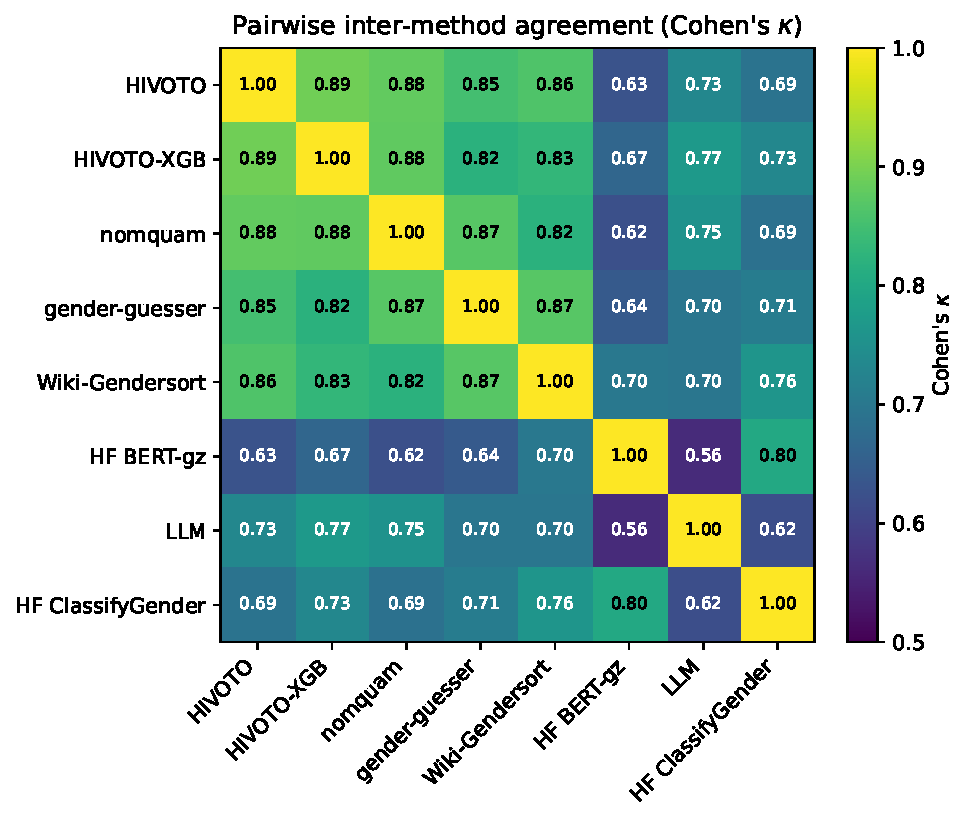
\includegraphics[width=0.85\linewidth]{figures/kappa_heatmap.pdf}
  \caption{Pairwise inter-method agreement (Cohen's $\kappa$) on the schleiermacher digital register. Three internally tight clusters are visible (HIVOTO/HIVOTO-XGB/nomquamgender, the dictionary methods gender-guesser/Wiki-Gendersort, and the two transformers); the LLM sits apart from all three. GND and the parenthetical-qualifier rule are excluded because their coverage overlap with the name-based methods is too small for a stable pairwise estimate.}
  \label{fig:kappa-heatmap}
\end{figure}

\begin{table}[h]
  \centering
  \scriptsize
  \setlength{\tabcolsep}{4pt}
  \begin{tabular}{lrrrrrrrr}
    \toprule
     & HV & HV-XGB & NQG & GG & WGS & HF-gz & LLM & HF-DB \\
    \midrule
    HIVOTO          & ---  & 0.89 & 0.88 & 0.85 & 0.86 & 0.63 & 0.73 & 0.69 \\
    HIVOTO-XGB      &      & ---  & 0.88 & 0.82 & 0.83 & 0.67 & 0.77 & 0.73 \\
    nomquamgender   &      &      & ---  & 0.87 & 0.82 & 0.62 & 0.75 & 0.69 \\
    gender-guesser  &      &      &      & ---  & 0.87 & 0.64 & 0.70 & 0.71 \\
    Wiki-Gendersort &      &      &      &      & ---  & 0.70 & 0.70 & 0.76 \\
    HF BERT-gz      &      &      &      &      &      & ---  & 0.56 & 0.80 \\
    LLM             &      &      &      &      &      &      & ---  & 0.62 \\
    HF DistilBERT   &      &      &      &      &      &      &      & ---  \\
    \bottomrule
  \end{tabular}
  \caption{Pairwise Cohen's $\kappa$ values underlying Figure~\ref{fig:kappa-heatmap}. HV~=~HIVOTO, NQG~=~nomquamgender, GG~=~gender-guesser, WGS~=~Wiki-Gendersort, HF-gz~=~HuggingFace BERT-genderize, HF-DB~=~HuggingFace DistilBERT.}
  \label{tab:kappa-matrix}
\end{table}

\paragraph{Per-record agreement.}
The aggregate $\kappa$ values quantify how much the methods agree \emph{on average}, but for editorial triage we need to know on \emph{which} entries they disagree. For every register entry we therefore additionally compute Fleiss' $P_i$, the per-item agreement component of Fleiss' $\kappa$, together with the Shannon entropy $H_i$ of the label distribution across the methods. Both summarise the same underlying vote distribution: $P_i$ measures how concentrated the votes are on a single label (1.0 = unanimous, lower bound = uniform across labels), and $H_i$ measures how dispersed they are. From these two values each entry is sorted into one of six tiers --- \texttt{unanimous}, \texttt{strong\_majority} (off by at most one method), \texttt{weak\_majority}, \texttt{no\_consensus}, \texttt{single\_rater}, and \texttt{no\_answer} --- which are exactly the tiers exposed to the editor in the review interface as a triage signal.

On the Schleiermacher register, this triage is heavily right-skewed: of the $8{,}277$ entries, $4{,}441$ ($53.7\%$) fall into the \texttt{unanimous} tier and a further $2{,}982$ ($36.0\%$) into \texttt{strong\_majority}. Only $492$ entries ($5.9\%$) land in \texttt{weak\_majority} and $362$ ($4.4\%$) in \texttt{no\_consensus} --- together $854$ entries (roughly one in ten) on which the bank cannot agree, and which the review interface surfaces first. The skew is also informative by majority label (Table~\ref{tab:tier-by-label}): where the methods settle on \texttt{male}, $80.8\%$ of entries are unanimous (mean $P_i = 0.93$); where they settle on \texttt{female}, $56.8\%$ are unanimous (mean $P_i = 0.84$); and entries the bank can only push into \texttt{ambiguous} are never unanimous (mean $P_i = 0.40$). The asymmetry between \texttt{male} and \texttt{female} agreement is itself a finding we return to in \S[TODO: discussion section]. Figure~\ref{fig:agreement-tiers} visualises the same data as a stacked-bar breakdown.

\begin{table}[h]
  \centering
  \small
  \begin{tabular}{lrrrrr}
    \toprule
    Majority label & $N$ & unanimous & strong\_maj. & weak\_maj. & no\_consensus \\
    \midrule
    \texttt{male}      & $4{,}548$ & $3{,}677$ ($80.8\%$) & $524$ ($11.5\%$) & $216$ ($4.7\%$) & $131$ ($2.9\%$) \\
    \texttt{female}    & $1{,}346$ & $764$ ($56.8\%$)     & $314$ ($23.3\%$) & $213$ ($15.8\%$) & $55$ ($4.1\%$)  \\
    \texttt{ambiguous} & $240$     & $0$ ($0.0\%$)        & $5$ ($2.1\%$)    & $59$ ($24.6\%$)  & $176$ ($73.3\%$) \\
    \bottomrule
  \end{tabular}
  \caption{Per-record agreement tier broken down by the majority label. The methods agree much more readily on \texttt{male} than on \texttt{female}; entries pushed to \texttt{ambiguous} are never unanimous and dominate the editorial review queue. (The remaining $2{,}143$ entries with $n_{\text{answered}} \le 1$ fall into \texttt{single\_rater} or \texttt{no\_answer} and are omitted.)}
  \label{tab:tier-by-label}
\end{table}

\begin{figure}[h]
  \centering
  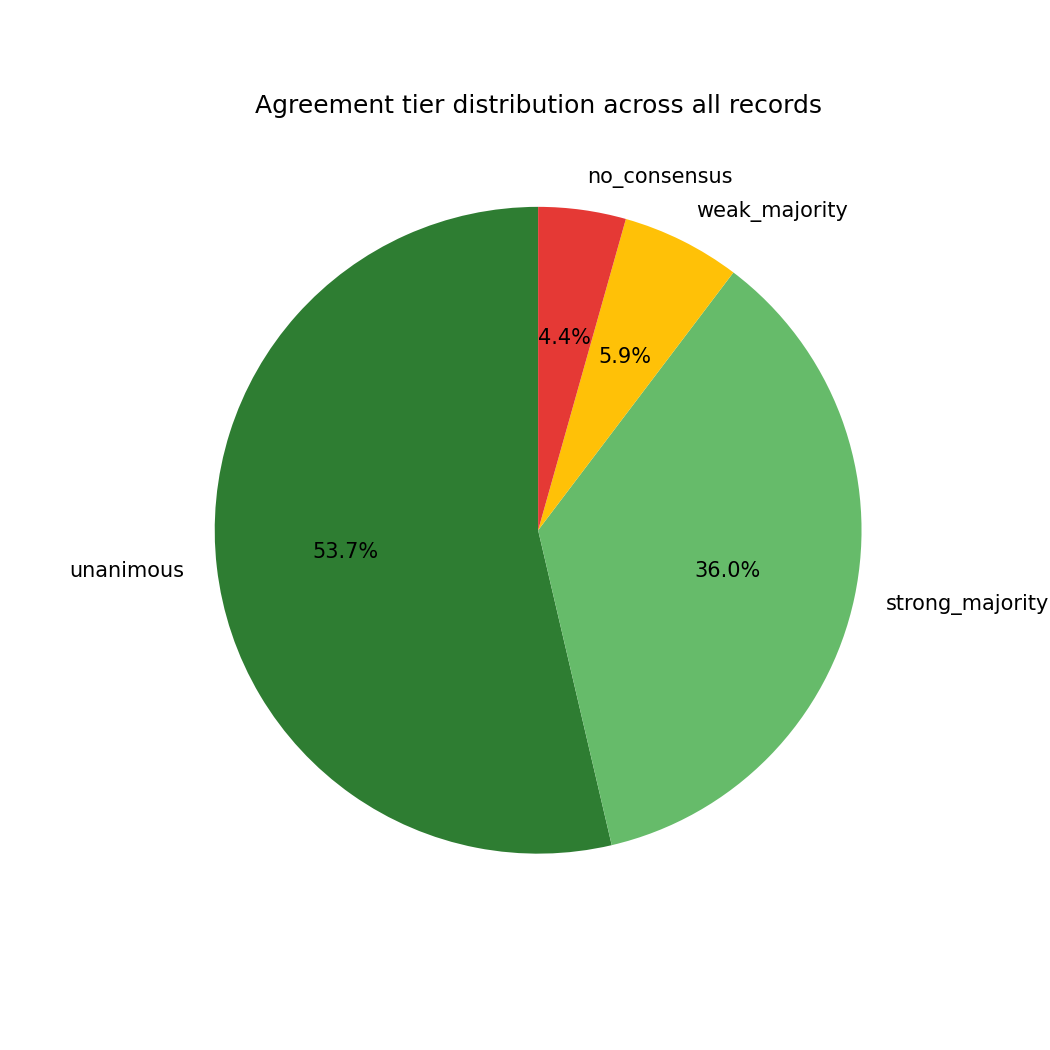
\includegraphics[width=0.85\linewidth]{figures/record_agreement_tiers.png}
  \caption{Per-record agreement tiers, segmented by the majority label assigned by the bank. The yellow \texttt{unanimous} band dominates the \texttt{male} column; the \texttt{female} column is more evenly split across tiers; and \texttt{ambiguous} entries cluster in the lower (less-agreed) tiers. The $P_i$ and $H_i$ distributions underlying these tiers are shown in Figure~\ref{fig:agreement-distributions}.}
  \label{fig:agreement-tiers}
\end{figure}

\begin{figure}[h]
  \centering
  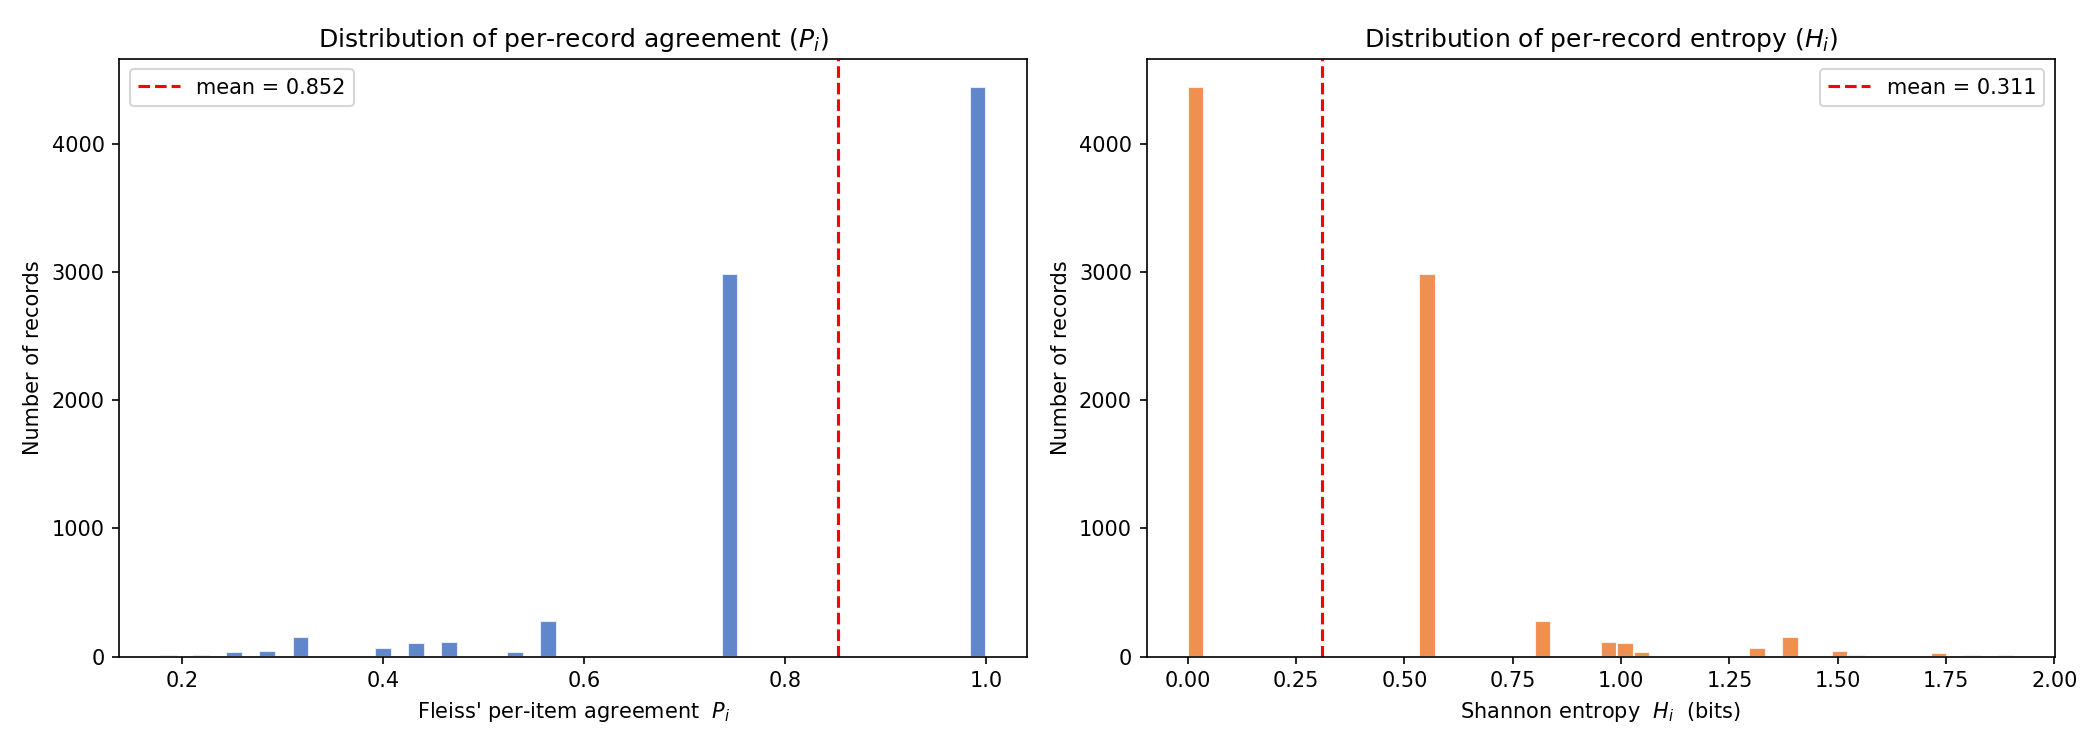
\includegraphics[width=0.85\linewidth]{figures/record_agreement_distributions.png}
  \caption{Distributions of Fleiss' per-item agreement $P_i$ (left) and Shannon entropy $H_i$ (right) across the $8{,}277$ register entries. Both distributions are strongly bimodal: most entries are close to unanimity ($P_i \to 1$, $H_i \to 0$), with a long thin tail of contested entries that drives the editorial review queue.}
  \label{fig:agreement-distributions}
\end{figure}

For the entries that fall into \texttt{no\_consensus} and \texttt{weak\_majority}, manual inspection of the most-contested records shows that disagreement clusters around four recurring profiles:

\begin{enumerate}
  \item Institutional names mis-parsed as personal names (\eg{} corporate correspondents).
  \item Initials-only entries, where dictionary methods have nothing to match against.
  \item Non-German names lying outside the coverage of the dictionary-based classifiers.
  \item Historically ambiguous names whose gendered usage shifted between the eighteenth and twenty-first centuries --- a problem that modern training data inherently amplifies.
\end{enumerate}

These are precisely the entries flagged for editorial review: disagreement functions as a triage signal, directing editor attention to cases where automated annotation is least reliable.

\subsection{Output Categories}

genderTagger uses four output categories: \texttt{male}, \texttt{female}, \texttt{uncertain}, and \texttt{institution}. The binary main classification reflects what name-based methods can in principle resolve --- a statistical association between historical name forms and implied gender. Non-binary, trans, and agender identities are not addressable from name strings alone and are deliberately not represented as classifier output categories. This is a limit we record rather than work around: the tool documents what it does not know, in the same spirit that \texttt{@cert} records what it is uncertain about. We return to this question in \S[TODO: discussion / limitations section].

\section{Case Study: schleiermacher digital}
\label{sec:case-study}

The development of genderTagger was conducted in collaboration with the \emph{schleiermacher digital} edition, which provides digital access to the correspondence, lectures, and diaries of the theologian Friedrich Schleiermacher (1768--1834).
% [FEHLT: kurze Beschreibung der Edition und ihres wissenschaftlichen Kontexts]

\paragraph{The register.} The edition's person register contains $8{,}277$ entries at the time of writing. Only $2{,}253$ of those entries ($27.2\%$) carry a GND identifier resolvable to a gendered authority record; the remaining $6{,}024$ entries ($72.8\%$) require alternative classification approaches. This distribution is representative of the practical limits of authority-file-based enrichment for a register of this size and historical scope: even a relatively well-curated GND attachment leaves nearly three quarters of the entries without an authoritative gender signal, motivating the multi-method approach described in \S\ref{sec:aggregation}.

\paragraph{Coverage per method.} Coverage on the Schleiermacher register varies systematically with each method's input requirements (Table~\ref{tab:coverage}). The local LLM, which receives the full register entry including biographical note, is the only method that produces a label for every entry. The five name-based classifiers --- gender-guesser, the two transformers, HIVOTO, and nomquamgender --- each cover the same $6{,}134$ entries ($74.1\%$): the gap to full coverage is exactly the set of entries with no usable forename. Wiki-Gendersort covers a slightly smaller subset ($73.4\%$) because its dictionary is more restrictive on non-Latin script and rare forms. The parenthetical-qualifier rule reaches $33.5\%$ of entries --- almost entirely because Schleiermacher's correspondents include a substantial number of women identified in the source through their relationship to a male principal (\textit{Frau des \dots}, \textit{Schwester von \dots}), a pattern the rule captures explicitly.

\paragraph{Per-method label distributions.} Coverage tells us only how often each method commits to \emph{some} label; the per-method label distribution (Table~\ref{tab:method-distribution}) shows \emph{which} labels each method tends to assign, and exposes systematic bias profiles that the aggregate $\kappa$ values smooth over. Three patterns are worth highlighting. First, the GND-matched subset is itself strongly skewed: of the $2{,}253$ entries with a usable GND record, $90.9\%$ resolve to \texttt{male} and only $9.1\%$ to \texttt{female} --- a more extreme imbalance than any name-based method produces. Second, the two HuggingFace transformers diverge markedly on the same $6{,}134$-entry coverage set: HF BERT-genderize predicts $\sim$$5\times$ as many \texttt{male} as \texttt{female} entries ($56.2\%$ vs.\ $11.2\%$), while HIVOTO on the identical input predicts only $\sim$$3\times$ as many ($53.3\%$ vs.\ $17.6\%$). The HF Genderize bias toward \texttt{male} is the dominant source of its low $\kappa$ against the LLM (Table~\ref{tab:kappa-matrix}). Third, the parenthetical-qualifier rule is the only method whose label distribution is approximately gender-balanced ($13.7\%$ \texttt{male} vs.\ $14.0\%$ \texttt{female}); this reflects the fact that it fires almost exclusively on relational descriptors, which in this corpus are predominantly used to identify women.

\begin{table}[h]
  \centering
  \scriptsize
  \setlength{\tabcolsep}{3pt}
  \begin{tabular}{lrrrrr}
    \toprule
    Method & male & female & inst. & unknown & abstain \\
    \midrule
    GND                  & $2{,}048$ ($24.7\%$) & $205$ ($2.5\%$)     & $0$ ($0.0\%$)   & $0$ ($0.0\%$)     & $6{,}024$ ($72.8\%$) \\
    Parenth.\ qualifier  & $1{,}133$ ($13.7\%$) & $1{,}159$ ($14.0\%$) & $7$ ($0.1\%$)   & $472$ ($5.7\%$)   & $5{,}506$ ($66.5\%$) \\
    gender-guesser       & $4{,}332$ ($52.3\%$) & $1{,}278$ ($15.4\%$) & $0$ ($0.0\%$)   & $524$ ($6.3\%$)   & $2{,}143$ ($25.9\%$) \\
    Wiki-Gendersort      & $4{,}457$ ($53.8\%$) & $1{,}292$ ($15.6\%$) & $0$ ($0.0\%$)   & $326$ ($3.9\%$)   & $2{,}202$ ($26.6\%$) \\
    HIVOTO               & $4{,}413$ ($53.3\%$) & $1{,}457$ ($17.6\%$) & $0$ ($0.0\%$)   & $264$ ($3.2\%$)   & $2{,}143$ ($25.9\%$) \\
    nomquamgender        & $4{,}379$ ($52.9\%$) & $1{,}380$ ($16.7\%$) & $0$ ($0.0\%$)   & $375$ ($4.5\%$)   & $2{,}143$ ($25.9\%$) \\
    HF BERT-gz           & $4{,}653$ ($56.2\%$) & $926$ ($11.2\%$)     & $0$ ($0.0\%$)   & $555$ ($6.7\%$)   & $2{,}143$ ($25.9\%$) \\
    HF DistilBERT        & $4{,}569$ ($55.2\%$) & $1{,}117$ ($13.5\%$) & $0$ ($0.0\%$)   & $448$ ($5.4\%$)   & $2{,}143$ ($25.9\%$) \\
    LLM                  & $5{,}426$ ($65.6\%$) & $1{,}897$ ($22.9\%$) & $119$ ($1.4\%$) & $835$ ($10.1\%$)  & $0$ ($0.0\%$)        \\
    \midrule
    \textbf{Combined}    & $5{,}452$ ($65.9\%$) & $1{,}867$ ($22.6\%$) & $83$ ($1.0\%$)  & $875$ ($10.6\%$)  & $0$ ($0.0\%$)        \\
    \bottomrule
  \end{tabular}
  \caption{Per-method label distributions on the Schleiermacher register ($N = 8{,}277$). Percentages are over the full register (so \texttt{abstain} = $1$ minus the coverage in Table~\ref{tab:coverage}). The combined row is the output of the aggregation pipeline (\S\ref{sec:aggregation}).}
  \label{tab:method-distribution}
\end{table}

\begin{table}[h]
  \centering
  \small
  \begin{tabular}{lrr}
    \toprule
    Method & Coverage & Share \\
    \midrule
    Local LLM (gpt-oss:20b)        & $8{,}277$ & $100.0\%$ \\
    gender-guesser                 & $6{,}134$ & $74.1\%$  \\
    HIVOTO                         & $6{,}134$ & $74.1\%$  \\
    HF DistilBERT (padmajabfrl)    & $6{,}134$ & $74.1\%$  \\
    HF BERT-genderize (imranali291)& $6{,}134$ & $74.1\%$  \\
    nomquamgender                  & $6{,}134$ & $74.1\%$  \\
    Wiki-Gendersort                & $6{,}075$ & $73.4\%$  \\
    Parenthetical-qualifier rule   & $2{,}771$ & $33.5\%$  \\
    GND authority lookup           & $2{,}253$ & $27.2\%$  \\
    \bottomrule
  \end{tabular}
  \caption{Per-method coverage on the schleiermacher digital person register ($N = 8{,}277$). Coverage is the number of entries on which the method returned a substantive label (not an abstention).}
  \label{tab:coverage}
\end{table}

\paragraph{Per-method accuracy against GND.} Treating the $2{,}253$ entries with a gendered GND authority record as a benchmark set allows a direct comparison of per-method classification quality (Figure~\ref{fig:benchmark-recall}). Effective accuracy --- correct labels divided by the full benchmark size, so abstentions count against the method --- ranges from $86.5\%$ (the two transformer classifiers, which abstain on $\sim$$12\%$ of the benchmark) to $99.7\%$ (the local LLM, which answers on every entry). The more revealing axis is the imbalance between male and female recall. The two transformer classifiers achieve $88$--$89\%$ on male names but only $60$--$71\%$ on female names, the largest per-class gaps in the cohort; gender-guesser, Wiki-Gendersort, HIVOTO, and nomquamgender close the gap considerably ($85$--$91\%$ female recall against $88$--$90\%$ male); only the LLM is balanced across classes ($99.7\%$ male, $100\%$ female on the GND benchmark). The benchmark itself is small and male-dominated ($2{,}048$ male vs.\ $205$ female), so female-recall figures should be read as ordinal rather than absolute, but the ordering is consistent with the disagreement profiles in \S\ref{sec:agreement}: methods with weaker female recall are also the methods that contribute disproportionately to the contested entries on female names.

\begin{figure}[h]
  \centering
  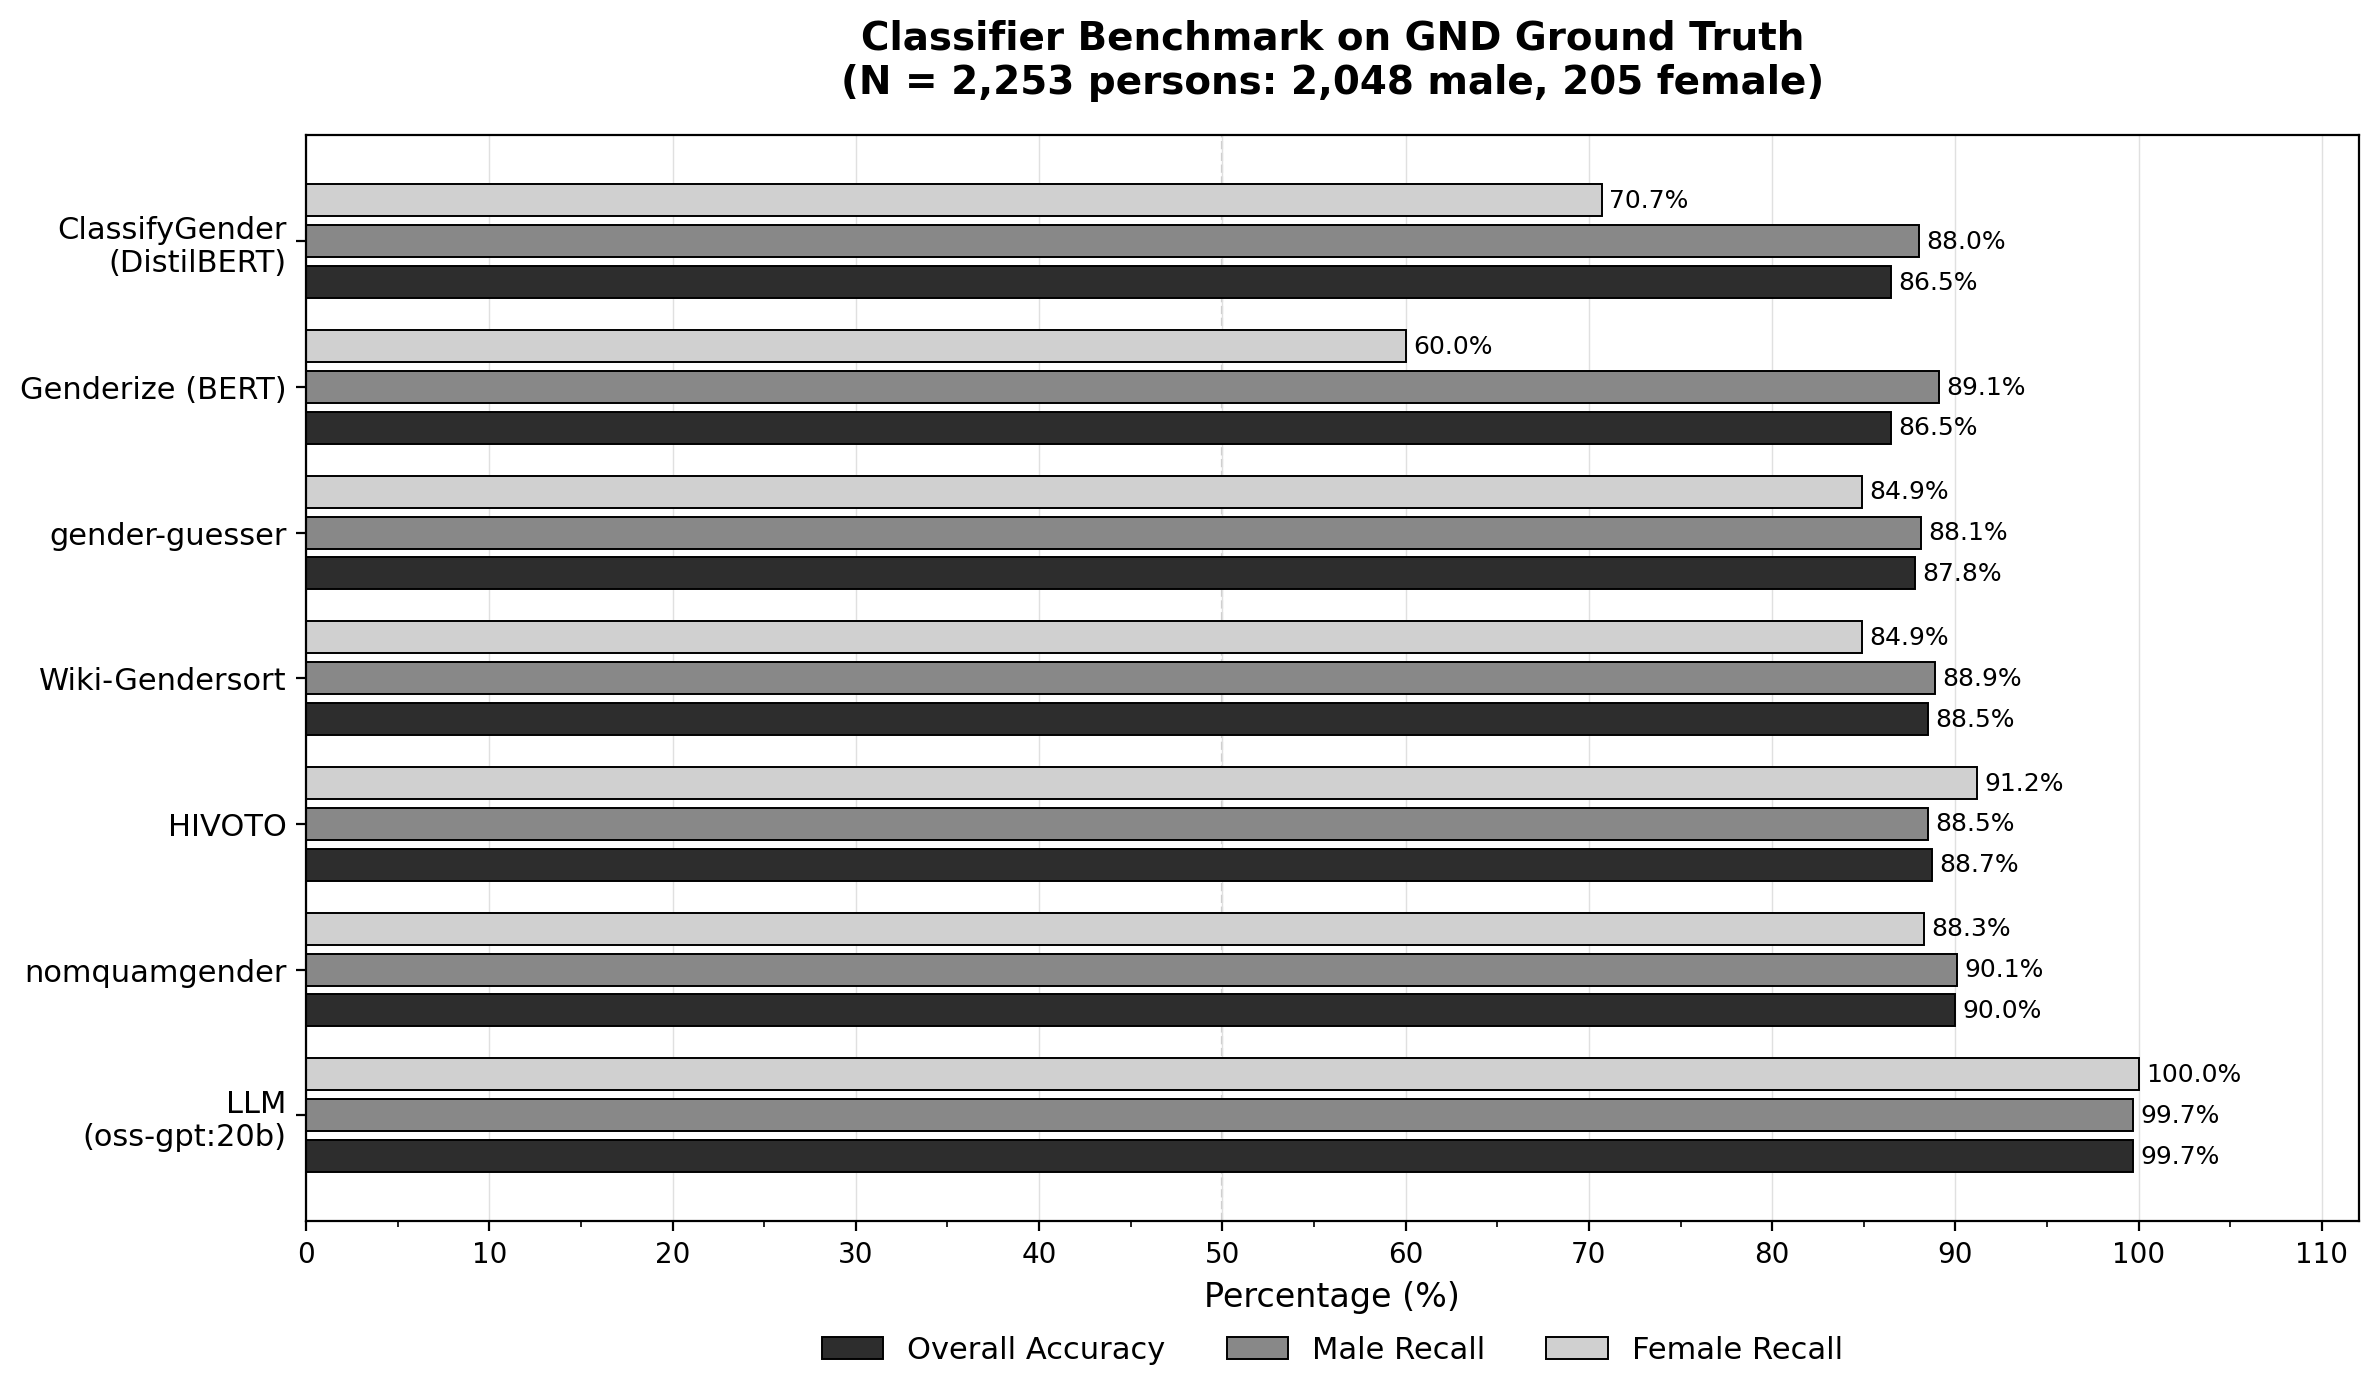
\includegraphics[width=\linewidth]{figures/benchmark_recall.png}
  \caption{Per-method effective accuracy and per-class recall on the Schleiermacher GND benchmark subset ($N = 2{,}253$ persons; $2{,}048$ male, $205$ female). Effective accuracy counts abstentions as errors, which is why the transformer classifiers --- despite high precision when they do answer --- score below the dictionary methods. The female-recall column shows the largest spread between methods.}
  \label{fig:benchmark-recall}
\end{figure}

\paragraph{Where methods disagree.} The disagreement profiles introduced in \S\ref{sec:agreement} appear at meaningful scale on this register. Of the $8{,}277$ entries, $854$ ($10.3\%$) fall into the \texttt{weak\_majority} or \texttt{no\_consensus} tiers and constitute the editorial review queue. Manual inspection of the most-contested entries shows that the four disagreement profiles --- institutional names mis-parsed as personal names, initials-only entries, non-German forms, and historically ambiguous names --- are not evenly distributed: the top contested records are dominated by entries where the source itself encodes a relationship rather than an independent identity (\eg{} \textit{(Frau des F.)}, \textit{(Sohn der Manon)}) and by initials-only references that defeat every name-based method.

% [FEHLT: ausgewählte konkrete Beispiele für jede der vier Konfliktklassen]

\paragraph{Resulting gender distribution.} The combined classification yields a strongly imbalanced distribution: of the $8{,}277$ entries, $5{,}452$ ($65.9\%$) are labelled \texttt{male}, $1{,}867$ ($22.6\%$) \texttt{female}, $83$ ($1.0\%$) \texttt{institution}, and $875$ ($10.6\%$) remain \texttt{unknown}. The male-to-female ratio of roughly $2.9{:}1$ is itself a finding about the source rather than about the method: a private and academic correspondence of an early-nineteenth-century Berlin theologian skews structurally toward male correspondents (university colleagues, ecclesiastical and political officeholders, publishers). The agreement evidence corroborates this: the methods agree unanimously on $80.8\%$ of the \texttt{male} entries but only on $56.8\%$ of the \texttt{female} entries (\S\ref{sec:agreement}), suggesting that the \texttt{female} category is both smaller in absolute terms and harder to assign reliably --- in part because women in this corpus are disproportionately referenced through relational descriptors that name-based methods cannot resolve.

% [FEHLT: Diskussion der Aussagekraft dieser Zahlen --- Verzerrung im Quellenmaterial vs.\ Verzerrung in den Methoden]

\begin{figure}[h]
  \centering
  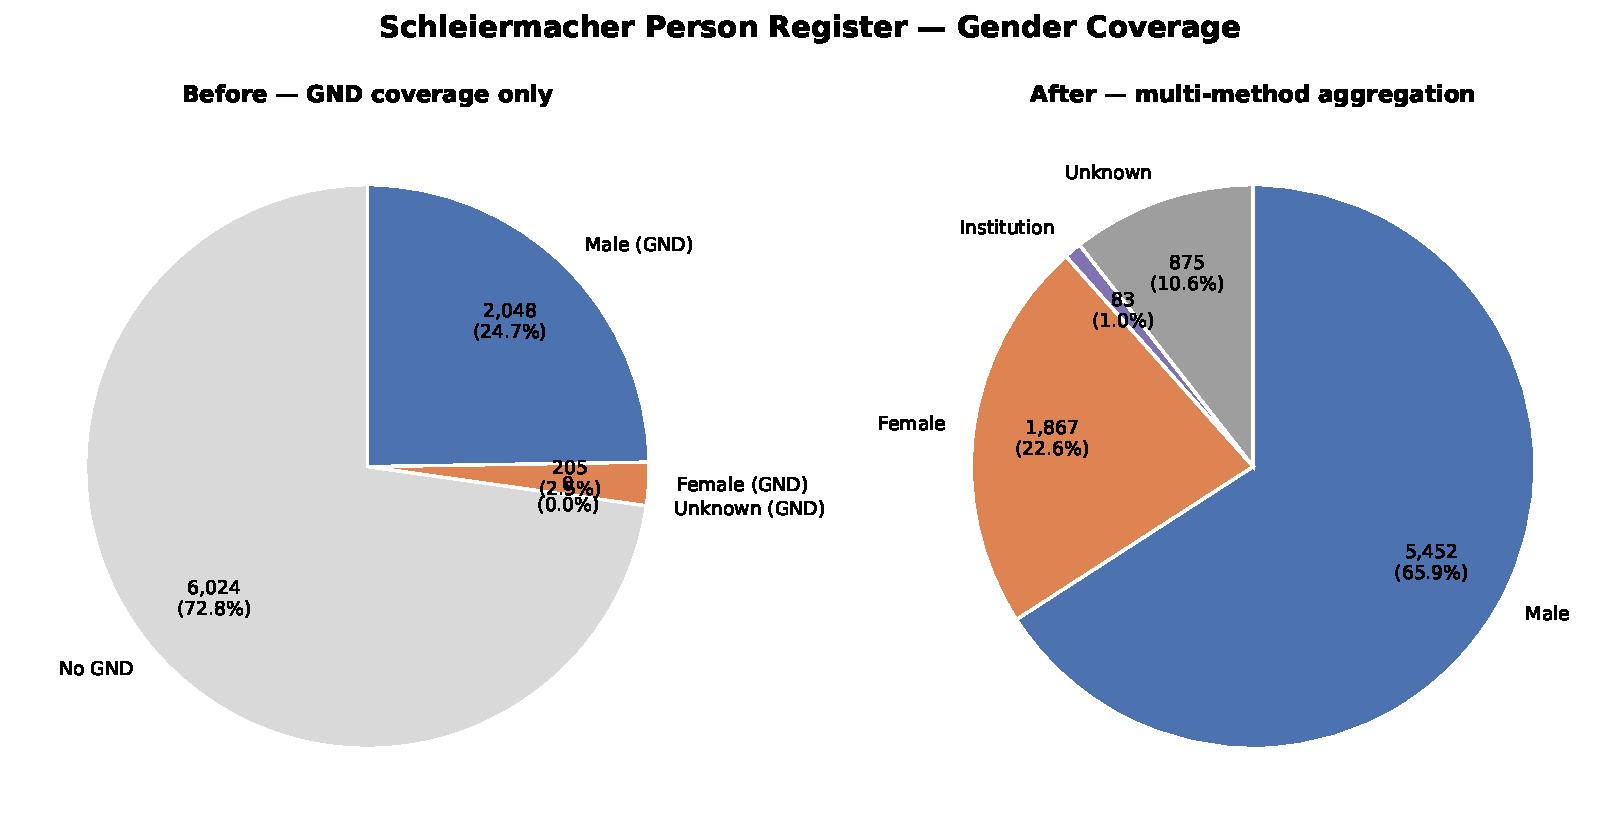
\includegraphics[width=\linewidth]{figures/gender_coverage_pies.pdf}
  \caption{Gender coverage of the Schleiermacher person register ($N = 8{,}277$) before and after multi-method aggregation. \emph{Left}: GND-only baseline --- $72.8\%$ of entries have no resolvable authority record. \emph{Right}: combined output of the aggregation pipeline (\S\ref{sec:aggregation}); every entry receives a label, with the residual \texttt{unknown} category restricted to entries on which the methods either abstained or could not reach consensus.}
  \label{fig:gender-pies}
\end{figure}

\paragraph{Lessons for comparable editions.} The case study suggests three transferable observations for editorial projects in a similar position. First, GND coverage alone is unlikely to suffice for any nineteenth-century or earlier register of comparable size; the long tail of non-authority entries demands a fallback strategy. Second, multi-method agreement provides not only a label but a meaningful triage signal: the $\sim$$10\%$ of entries on which the methods cannot agree concentrates exactly the cases where editorial attention is most warranted. Third, source-specific structural patterns --- in this register, the relational naming convention for women --- can be addressed by lightweight, edition-specific rules (the parenthetical-qualifier method here), provided the combination strategy is open enough to admit them as full peers of the off-the-shelf classifiers.

% [FEHLT: Reflexion: Übertragbarkeit auf andere Editionsprojekte mit anderem Sprach-/Zeitprofil]


\section{Human-in-the-Loop Workflow}
\label{sec:hitl}

Rather than treating automated classifications as definitive assignments, genderTagger is explicitly designed as a human-in-the-loop workflow in which editorial decisions remain subject to human interpretation and revision. A typical session runs:  \texttt{import TEI $\to$ batch-classify with all methods $\to$ inspect agreement and disagreement $\to$ annotate (confirm or override) $\to$ export}. Classifier execution is decoupled from the user interface: long-running methods such as transformer models and the local LLM run in the background, while editors can already begin reviewing entries that the faster methods have classified. This matters in practice --- running a 20-billion-parameter local LLM over several thousand register entries takes hours, and a blocking UI would make the tool unusable on registers of realistic size.

The locally operated language model achieved comparatively higher classification accuracy by incorporating contextual information from the TEI \verb|<note>| elements; however, these contextual descriptions are themselves the result of prior editorial research and interpretation, meaning that existing editorial biases may already be embedded in the source material and subsequently reproduced through the model’s classifications. 

% [FEHLT: Workflow-Diagramm (Import -> Klassifikation -> Triage über Agreement -> Review/Override -> Export) als Abbildung]
% [FEHLT: Beschreibung der konkreten editorischen Review-Prozesse: Wer entscheidet wann? Vier-Augen-Prinzip? Umgang mit \texttt{cert="low"}-Einträgen? Versionierung der editorischen Overrides?]


\section{Conclusion and Future Work}
\label{sec:conclusion}

genderTagger demonstrates how semi-automated gender annotation can support metadata enrichment workflows in TEI/XML-based digital editions while preserving editorial oversight and interpretative responsibility. By combining multiple classification methods, integrating uncertainty-aware review mechanisms, and embedding annotation directly into existing editorial infrastructures, the system contributes both methodological and infrastructural perspectives to ongoing discussions surrounding bias, metadata enrichment, and human-centered AI in the Digital Humanities.

As geographer Joni Seager (2016) remarked, albeit in a different context: "what gets counted counts". The same applies in digital editions. If gender is not a category to be captured and explored, the imbalances it encodes remain invisible, and invisible imbalances cannot be analyzed or studied further. By building a genderTagger and integrating gender as a searchable category in the registers of digital editions, we take a small but meaningful step toward creating gender visibility.

If gender is a documented category, researchers can, for instance, systematically ask which women were part of a literary network, how often they were mentioned compared to their male contemporaries, and in what roles they appeared. They can also trace whether women and other marginalized groups wrote about different topics or in different styles, and whether those differences reflect genuine creative choices or the constraints imposed on them by society. All these are further researches which only can be carried out if gender is modelled in the first place.

But the implications reach beyond academic research. When gender becomes a legible category in our digital cultural heritage, it sends a signal about what we consider worth knowing. It insists that the stories of women and other marginalized groups are not footnotes to history, but part of its fabric. And it gives future readers the tools to ask questions that previous generations simply could not.

% [FEHLT: klare Zusammenfassung der wichtigsten Ergebnisse]

Future work will focus on expanding multilingual support, improving explainability and confidence estimation, integrating additional authority data sources such as Wikidata, and exploring adaptive learning approaches based on editorial feedback.

% [FEHLT: evtl. Open Source/GitHub/Verfügbarkeit erwähnen]


% Acknowledgements for colleagues, referees, ...
% ==============================================
\begin{acknowledge}
KD acknowledges support by DFG Project \geprislink{000000000}.
\end{acknowledge}

\begin{data}
My data is publicly available on zenodo.
\end{data}

\begin{aiuse}
No AI hallucinations over here.
\end{aiuse}

% Bibliography with BibTeX
% ========================
\bibliographystyle{eceasst}
\bibliography{gendertagger}

\end{document}
